% !TeX root = ../notes.tex

\section{Textbook Query Optimization}
Textbook query optimization involves techniques to perform a rough first optimization, which however is quite simple. There is a series of steps to translate raw SQL into logical and physical plans, each of them transforming input in a more optimal form.

The output is going to be executable, but still to be improved by non-trivial methods.

\subsection{Algebra and tuples}
Plain relational algebra is not sufficient itself: it needs to be revisited ensuring correctness (producing the same result) within a formal model. The most relevant problem to tackle is deciding whether two algebraic expressions are the same, but this in difficult in practice.

For instance, performing a selection before a join might be correct (and faster) in case the considered criterion is equality, but can give a different result than selecting after an outer join. 

To remedy this issue, it is possible to guarantee that two expressions are equivalent, not accepting false positing yet allowing false negatives. 

A formal definition of tuple is an unordered mapping from attribute names to values of a domain. A schema consists in a set of attributes with domain $A(t)$.

Tuple operations are:
\begin{itemize}
	\item Concatenation, attaching one tuple to another regardless of ordering (union);
	\item Projection, producing a notation $t.a$ in which it is possible to access single values or multiple $t_{|\{a, b\}}$, getting a subset of the schema.
\end{itemize}

A set of tuples with the same schema forms a relation. Sets naturally do not comply with real data, since they not allow duplicates, but are used for simplicity.

In most cases, sets and bags can be used interchangeably, but the optimizer considers different semantics: logical algebra operates on bags, physical algebra on streams and sets are only considered after an explicit duplicate elimination.

Set operations are the classic ones of union, intersection and difference, yet are subject to schema constraints. On bags, operations are performed on frequencies. 

There are also free variables, which first must be bounded to be evaluated: they are essentials for predicates and algebra expressions, such as dependent joins. 

It is important to note that projection removes duplicates within sets, while keeping them in bags.

There are equivalences for selection and projection useful to derive whether a different ordering produces the same output. For instance, applying selection twice is the same as applying it once with two criteria plus an AND. Commutative property also holds.

\subsection{Canonical Query Translation}
The canonical query translation transforms SQL into algebra expressions. The first approach involves some restrictions: it assumes no duplicates without aggregation and set operations.

The first step is translating the FROM clause:
$$F = \begin{cases}
R_1 & k = 1 \\
((\dots (R_1 \times R_2) \times \dots) \times R_k)) & \text{else}
\end{cases}$$
In short all relations are joined through a cross product. The next step is translating the WHERE clause:
$$W = \begin{cases}
F & \text{there is no WHERE clause} \\
\sigma_p(F) & \text{otherwise}
\end{cases}$$
The SELECT clause is translated starting from the projection $a_1,\ \dots,\ a_n$ or $*$. The expression is constructed:
$$S = \begin{cases}
W & \text{if the projection is ALL} \\
\prod_{a_1,\ \dots,\ a_n}(W) & \text{otherwise}
\end{cases}$$
GROUP BY can also be translated, even though it is not part of the canonical translation. Let $g_1,\ \dots,\ g_n$ be the attributes in the clause and $agg$ the aggregations within SELECT:
$$G = \begin{cases}
W & \text{there is no GROUP BY clause} \\
\Gamma_{g_1,\ \dots,\ g_m:agg}(W) & \text{otherwise}
\end{cases}$$
HAVING is basically the same as WHERE, with the filter predicate on top of $G$.

\subsection{Logical Query Optimization}
Once obtained the relational algebra, equivalences span the potential search space and new expressions are derived thanks to them. Of course equivalence can be applied in both ways, hence it is relevant to decide which one works better, and conditions have to be checked as well. This, however, makes the search more expensive since there are plenty of alternatives.

To speed the process up, sometimes some equivalences are ignored, even the simplest ones (for instance when choosing the join algorithm).

Query plans can only be compared if there is a cost function, often needing details which are not available merely through relational algebra (what kind of join is being used): logical query optimization is still a heuristic and requires additional steps, since it is not enough to determine the runtime.

Most algorithms, therefore, use the following strategy:
\begin{itemize}
	\item Organization of equivalences into groups;
	\item Directing equivalences, deciding the preferred side and rewriting rules to apply them sequentially to the initial expression, trying to reduce the size of intermediate results.
\end{itemize}
For example, a projection on the output of a join can be preferred to a join of a projection. It is important to keep in mind that tuples are being removed in the process, and this only applies in certain circumstances (regular expressions, high selectivity of join).

The rule of thumb is simply to eliminate the most tuples during the intermediate step, to then perform computationally expensive operation with the smallest amount of data.

To summarize, the phases are:
\begin{itemize}
	\item Breaking up conjunctive selection predicates, since simpler predicates can be moved around easier;
	\item Pushing selections down, reducing the number of tuples early;
	\item Introducing joins, which are cheaper than cross product (linear time);
	\item Determining join order;
	\item Introducing and pushing down projections, removing redundant attributes.
\end{itemize}
Some SQL queries have limitations: selections sometimes cannot be pushed down, since there might be no join predicate between tables. Choosing a different join order allows further push down. 

\subsection{Physical Query Optimization}
Physical query optimization adds execution information to the plan, allowing actual cost calculation and optimizing over data structures, access path and operator implementation.

Data may be sorted or materialized, introducing results which can be reused and deciding where to store them.

First of all, the access path is selected: lookup can be done through index or table scan, depending on the selectivity (fraction of the data satisfying the clause): in general, above 10\% a table scan is recommended. 

Scanning a table might be efficient since tuples are stored adjacent in memory; using index, instead, involves traversing a tree multiple times starting from the root. 

Sometimes it is useful to just store in cache the output of a view, but that also depends on the query plan: intermediate results should actually be reused.

Operator selection is replacing a logical operator with a physical one, according to semantic restrictions (most operators require equi-join).

A blockwise nested loop join is generally better than a natural join; sort merge join and hash join are better than both. In general, hash join is the best if not reusing sorts. This process must be performed for all operators: sort join requires ordered tuples, distributed databases need local data and there are multiple ways to model the properties (hashing).

Sort merge join might outperform the hash join if the amount of data is much larger than the available memory.

Materializing, on the other side, is quite relevant for nested loop joins: the first pass is expensive, but the afterwards ones are way cheaper, making it essential for multiple consumers. 

\subsection{Join Ordering}
Join ordering focuses on conjunctive queries with simple predicates of the type $a_1 = a_2$ where the latter can be either an attribute or a constant (commonly algorithms assume join between attributes).

Relations may include selections or complex building blocks, however for simplicity filtering is ignored; having operators other than equality might cause differences within the query planner.

Ordering basically means choosing which relation to be joined first, placing entities in a graph and adding an edge whenever a predicate from a node is joined to another. 

This kind of schema is defined as a query graph, in which edges consist in predicates and self loops represent equality with a constant. Usually cycles are pushed down, since algorithms only assume attributes. 

Based on the query graph it is possible to obtain an overview of the complexity of the problem: there are different shapes which are treated differently. 

\begin{figure}[h]
	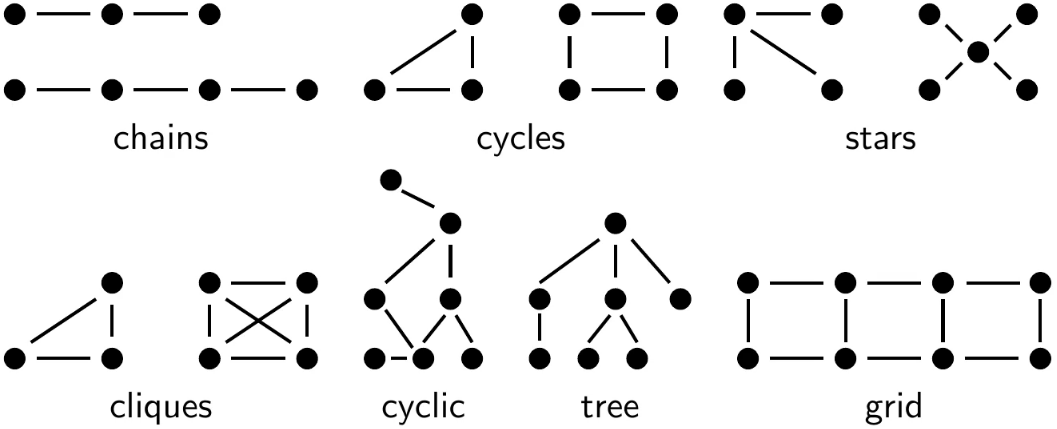
\includegraphics[scale=1.5]{query_graph.png}
	\centering
\end{figure}

\begin{enumerate}
	\item Chains are the simplest kind of query, fairly common in practice;
	\item Cycles (cyclic) are a chain with a closing edge, the easiest example of cycles;
	\item Stars are mostly used in data warehouse, in which the center table has large dimension and the ones outside are relatively small, quite different to solve;
	\item Cliques are instances in which every relation is joined with all the others, and are the hardest to optimize causing the worst runtime;
	\item Trees are acyclic queries even if the level of nesting can be high;
	\item Grids are also fairly hard and interesting for research.
\end{enumerate}

Joins are represented with join trees, binary trees with operators as inner nodes and relations as leaves. The most common type is unordered (not distinguish left from right) without cross product, however algorithms might produce other variants.

There furthermore are different kinds of trees:
\begin{itemize}
	\item Left-deep tree, in which joins only happen on the left side, easy to represent and implement through hash tables ($n!$ trees with cross products);
	\item Right-deep tree ($n!$);
	\item Zig-zag tree, a combination of the previous ($n!2^{n-2}$);
	\item Bushy tree, a full binary tree (non-linear, harder to find optimal solutions but can be the most efficient in some cases, $n!C(n-1) = \frac{(2n-2)!}{(n-1)!}$ where $C$ represents a Catalan number).
\end{itemize}
It is relevant to notice that the number of leaf combinations and unlabeled trees grows exponentially, and increases even more with a flexible structure. However, nodes can often be swapped from left to right.

Another important information about joins is their selectivity: 
$$f_{i, j} = \frac{\abs{R_i \bowtie_{p_{i, j}} R_j}}{\abs{R_i \times R_j}}$$
This depends on whether the attributes are a key, and gives an estimation of the result cardinality with the aid of assumptions and statistics.

Given a join tree, the cardinality can be computed recursively as the productory of the selectivity function multiplied by the size of both relations. This allows easy calculations only requiring base cardinalities and independence of predicates:
$$C_{out}(T) = \begin{cases}
0 & T\text{ is a leaf} \\
\abs{T} + C_{out}(T_1) + C_{out}(T_2) & T = T_1 \bowtie T_2
\end{cases}$$
This formula sums up the sizes of intermediate results, which are the ones causing more works. There are basic specific cost functions for joins, to be summed to the cost of single relations. 

Algorithms are mainly designed for left-deep trees, and some of the cost functions do not work in practice, for instance in the case of cross products. Therefore, those indicators are mainly theoretical and work under strict assumptions. However, join ordering is a main factor regardless of the chosen cost methods.

A cost function is called symmetric if $C_{impl}(e_1 \bowtie^{impl} e_2) = C_{impl}(e_2 \bowtie^{impl} e_1)$. Commutativity can be ignored.

Most of the time, algorithms for query optimization tend to avoid cross products, despite the enormous number of possibilities to build a join tree: the only exception regards small relations.

\subsubsection{Chains}
Chains usually originate a left-deep tree: leaves can be ordered according to different degrees of freedom, as long as all the relations are joined. 

The number of possible left-deep trees can be defined recursively:
$$\begin{cases}
f(0) = 0 \\
f(1) = 1 \\
f(n) = 1 + \sum_{k=1}^{n-1} f(k-1) \cdot (n - k)
\end{cases}$$
Adding $R_n$ to all possible join trees can be done at any position following $R_{n-1}$. There are $n - k$ join trees for $R_n$, plus one assuming it can be placed before $R_{n-1}$ in the case of $k=1$. For $R_{n-1}$ to be at $k$, $R_{n-k} - \dots R_{n-2}$ must be below it.

Solving the recurrence gives the closed form $f(n) = 2^{n-1}$, still exponential yet much less than the case with cross products.

A generalization to zig-zag can be made expecting the same result.

Bushy trees, on the other hand, are not so easy to obtain: each subtree must contain a subchain to avoid cross products, hence single relations should not be added. It is possible to create a whole chain $R_1 - \dots R_n$, cut it and place it under another subtree, always considering commutativity.

This gives the formula:
$$ f(n) = \begin{cases}
1 & n < 2 \\
\sum_{k=1}^{n-1} 2f(k) \cdot f(n-k) & n \geq 2
\end{cases}$$
Having more than 2 relations implying performing a cut at some point $k$ and placing $k$ on the left side, $n - k$ on the right side. A factor of 2 indicates swapping the two sides. 

This gives the closed form $f(n) = 2^{n-1}C(n-1)$.

\subsubsection{Stars}
Star queries have the constraint that one relation must be in the center; all the others can be ordered arbitrarily. This leads to the following formulas:
\begin{itemize}
	\item Left-deep: $2 \cdot (n - 1)!$, since there are $n - 1$ choices for a join partner and a factor of 2 for commutativity;
	\item Zig-zag: $2 \cdot (n - 1)! \cdot 2^{n-2}$, in which the last factor represent the possibility to swap left and right for each subtree;
	\item Bushy trees: not possible since they require the first relation to be available. 
\end{itemize}

\subsubsection{Cliques}
Cliques are a schema which do not care about cross products, since every relation is connected to the other, hence the number of possibilities is the same as the one obtained allowing cross products. 

Still, complexity is very high and runtime is bad, although the worst case usually does not happen. 

\subsection{Greedy heuristics}
Regardless of the methods and the inclusion of cross products, the search space is in general quite large when the number of relations is larger than 10, and polynomial time is hard to achieve. Some cost functions do not even have a proof of complexity.

Due to the size of the search space, greedy heuristics are ways to easily construct a potential tree in a fast time: they are most suitable for large queries, but often do not give the best result.

Algorithms assume no cross products within left-deep trees, and known cardinalities (or some other weight function).

\subsubsection{GreedyJoinOrdering-1}
This algorithm returns a set of ordered relations to be joined according to a cost function in a bushy tree structure. 

The output is given starting from the minimum-weight relation, removes it and searches for the new minimum. 

This method is simple, but not that good in practice: it assumed fixed weight (not depending on the size, for instance) and does not support optimization within intermediate results. 

\subsubsection{GreedyJoinOrdering-2}
This variant also considers the previous set of relations, computing relative weights based on the existing tree. 

In this case, however, the very first relation has a large relative weight and a major impact on the choices made afterwards. 

\subsubsection{GreedyJoinOrdering-3}
To tackle this problem, a double loop is introduced in which not only the set of relations is scanned, but also every relation is tested as a starting one. Then, all computed results are compared and the minimum among them is returned. 

This method is overall the best one and is implemented in some systems, but it is still not optimal.

\subsubsection{Greedy Operator Ordering}
Intermediate join trees must be combined to obtain larger trees: since some algorithms construct left-deep structures and others return bushy trees, those can be attached if the result is minimal.

Trees with the smallest weight are iteratively joined and then removed by the set of possibilities. 

\subsection{IKKBZ}
IKKBZ is a polynomial time algorithm for join ordering without cross products, producing left-deep trees under some assumptions: acyclic graphs, ASI cost functions and a fixed join technique.

The algorithm will ultimately compute a rank for each predicate, based on its selectivity, obtaining an optimal evaluation order. 

After the first steps, however, the remaining arguments are independent on the size of the relations.